\Section{accel}{GPU programming with \emph{Accelerate}}

\newcommand{\acc}{\textit{Accelerate}}

This section will be a brief introduction to using the
\acc{} framework for GPU programming.

Over the next few sections we will be introducing the various concepts
of \acc, illustrated by examples that you can type directly into GHCi.
These small examples will not be running on the GPU, instead they will
be using \acc's interpreter.  To play with examples yourself, first
make sure the @accelerate@ package is installed:

\begin{verbatim}
$ cabal install accelerate
\end{verbatim}

\noindent The @accelerate@ package provides the basic infrastructure:
the module @Data.Array.Accelerate@ for constructing array
computations, and @Data.Array.Accelerate.Interpreter@ for interpreting
them.  To actually run an \acc{} computation on a GPU you will also
need the @accelerate-cuda@ package, but we'll cover that later
(\secref{accel-gpu}).

Next, start up GHCi and import the necessary modules:

\begin{verbatim}
$ ghci
Prelude> import Data.Array.Accelerate as A
Prelude A> import Data.Array.Accelerate.Interpreter as I
Prelude A I> 
\end{verbatim}

\Subsection{accel-overview}{Overview}

\acc{} is a \emph{domain-specific language} for programming GPUs.
Programs are written in Haskell syntax using operations of the
framework, but the method by which the program runs is very different
from a conventional Haskell program.  Broadly speaking, a program
fragment that uses \acc{} works like this:

\begin{itemize}
\item The Haskell code generates a data structure in an internal
  representation that the programmer doesn't get to see,
\item This data structure is then either \emph{compiled} into GPU code
  and run directly on the GPU, or it can be \emph{interpreted} using
  \acc's built-in interpreter.  Both methods give the same results,
  but of course running on the GPU should be far faster.
\end{itemize}

By the magic of Haskell's overloading and abstraction facilities, the
Haskell code that you write using \acc{} usually looks very much like
ordinary Haskell code, even though it is generating a data structure
rather than actually evaluating the result directly.

While reading this tutorial you probably want to have a copy of the
\acc{} API documentation to hand: \url{http://hackage.haskell.org/packages/archive/accelerate/0.12.0.0/doc/html/Data-Array-Accelerate.html}.

\Subsection{accel-arrays}{Arrays and indices}

Everything in \acc{} revolves around arrays.  Arrays are the
fundamental datatype that we operate on: an \acc{} computation takes
arrays as inputs and delivers one or more arrays as output.

The type of arrays has two parameters:

\begin{haskell}
data Array sh e
\end{haskell}

\noindent where @e@ is the element type.  The @sh@ parameter
describes the \emph{shape} of the array, that is, the number
of dimensions.  Unlike the @Ix@ class that standard Haskell arrays are
paramterised over, the shape parameter is rather more flexible, as we
shall see.

Shapes are built out of two type constructors, @Z@ and @:.@

\begin{haskell}
data Z = Z
data tail :. head = tail :. head
\end{haskell}

For example, @Z@ is the shape of an array with no dimensions, i.e. a
scalar, which has a single element.  If we add a dimension, @Z :. Int@, this is the shape of an array with a single dimension indexed
by @Int@, otherwise known as a vector.  Adding another dimension gives
@Z :. Int :. Int@, the shape of two-dimensional arrays.  Note that new
dimensions are added on the right, and the rightmost index is the one
that ``varies the fastest''.

Remember that @Z@ and @:.@ are both type constructors and value
constructors; this can get a bit confusing at times.  For example, @Z :. 3@ has type @Z :. Int@.  The value form is used in \acc{} to mean
either ``sizes'' or ``indices''; for example, @Z :. 3@ can be either
the shape of 3-element vectors, or the index of the third element of a
vector.

A few handy type synonyms are provided for the common shape types:

\begin{haskell}
type DIM0 = Z
type DIM1 = DIM0 :. Int
type DIM2 = DIM1 :. Int
\end{haskell}

\noindent In fact, \acc{} only supports @Int@-typed indices, and indices
always begin at zero.  Since dimensionalities of zero and one are
common, the library provides type synonyms for those:

\begin{haskell}
type Scalar e = Array DIM0 e
type Vector e = Array DIM1 e
\end{haskell}

The library allows us to build arrays and experiment with them in
ordinary Haskell code, so let's try a few examples.  A simple way to
build an array is using @fromList@:

\begin{haskell}
fromList :: (Shape sh, Elt e) => sh -> [e] -> Array sh e
\end{haskell}

\noindent Don't worry about the @Shape@ and @Elt@ type classes, they
are just there to ensure that we only use the approved shape
constructors (@Z@ and @:.@) and approved element types respectively.

Let's build a 10-element vector of @Int@, and fill it with the numbers
$1\ldots10$.  We need to pass a shape argument, which will be @Z:.10@
for a 10-element vector:

\begin{verbatim}
> fromList (Z:.10) [1..10]
<interactive>:9:1:
    No instance for (Shape (Z :. head0))
      arising from a use of `fromList'
    Possible fix: add an instance declaration for (Shape (Z :. head0))
    In the expression: fromList (Z :. 10) [1 .. 10]
    In an equation for `it': it = fromList (Z :. 10) [1 .. 10]
\end{verbatim}

\noindent Oops!  This illustrates something that you will probably
 encounter a lot when working with \acc: a type error caused by
insufficient type information.  In this case, since integers are
overloaded in Haskell, we have to say explicitly that we mean @Int@
for the indices of our vector.  There are many ways to give GHC the
extra bit of information it needs, one way is to add a @Vector Int@
type signature to the whole expression:

\begin{verbatim}
> fromList (Z:.10) [1..10] :: Vector Int
Array (Z :. 10) [1,2,3,4,5,6,7,8,9,10]
\end{verbatim}

Similarly, we can make a two-dimensional array, with 3 rows of 5
columns:

\begin{verbatim}
> fromList (Z:.3:.5) [1..] :: Array DIM2 Int
Array (Z :. 3 :. 5) [1,2,3,4,5,6,7,8,9,10,11,12,13,14,15]
\end{verbatim}

\noindent Even though we've created a two-dimensional array, we
initialised it from a flat list, and it still looks like a flat list
when printed out.  In fact, all arrays are represented as flat lists
(after all, computer memory is one-dimensional).  The shape of the
array is only there to tell the library how to interpret the
operations on it---if we ask for the index @Z:.2:.1@ in an array with
shape @Z:.3:.5@ we'll get the element at position $2 \times 5 + 1$.
We can try it using @indexArray@:

\begin{verbatim}
> let arr = fromList (Z:.3:.5) [1..] :: Array DIM2 Int
> indexArray arr (Z:.2:.1)
12
\end{verbatim}

One thing to remember is that in \acc{}, arrays cannot be nested: it is
not possible to build an array of arrays.  This is because arrays must
be able to be mapped directly into flat arrays on the GPU, which has
no support for nested arrays.

We can, however, have arrays of tuples.  For example:

\begin{verbatim}
> fromList (Z:.2:.3) (Prelude.zip [1..] [1..]) :: Array DIM2 (Int,Int)
Array (Z :. 2 :. 3) [(1,1),(2,2),(3,3),(4,4),(5,5),(6,6)]
\end{verbatim}

Internally, \acc{} will translate an array of tuples into a tuple of
arrays; this is done entirely automatically and we don't need to worry
about it.  Arrays of tuples are a very useful structure as we shall
see.

\Subsection{accel-running}{Running a simple \acc{} computation}

So far we have been experimenting with arrays in the context of
ordinary Haskell code, we haven't constructed an actual \acc{}
computation over arrays yet.  An \acc{} computation takes the form
@run @$E$, where

\begin{haskell}
run :: Arrays a => Acc a -> a
\end{haskell}

\noindent and $E$ is an expression of type @Acc a@, which means ``an
accelerated computation that delivers a value of type @a@''.  The
@Arrays@ class allows @a@ to be either an array, or a tuple of
arrays. A value of type @Acc a@ is really a data structure (we'll see
in a moment how to build it), and the @run@ function evaluates the
data structure to produce a result.  There are two variants of @run@:
one exported by @Data.Array.Accelerate.Interpreter@ that we will be
using for experimentation and testing, and another exported by
@Data.Array.Accelerate.CUDA@ (in the @accelerate-cuda@ package) that
runs the computation on the GPU.

Let's try a very simple example.  Starting with the $3x5$ array of
@Int@ from the previous section, we will add one to every element:

\begin{verbatim}
> let arr = fromList (Z:.3:.5) [1..] :: Array DIM2 Int
> run $ A.map (+1) (use arr)
Array (Z :. 3 :. 5) [2,3,4,5,6,7,8,9,10,11,12,13,14,15,16]
\end{verbatim}

\noindent Breaking this down, first we call @A.map@, which is the
function that maps over arrays (we needed the @A.@ prefix to
disambiguate with @Prelude.map@; recall that we used
@import Data.Array.Accelerate as A@ earlier).

\begin{haskell}
A.map ::
  (Shape ix, Elt a, Elt b) =>
  (Exp a -> Exp b) -> Acc (Array ix a) -> Acc (Array ix b)
\end{haskell}

\noindent As its second argument, @A.map@ takes an @Acc (Array ix a)@,
whereas we have an @Array DIM2 Int@.  In order to get this array into
the @Acc@ world, we have to apply the function @use@:

\begin{haskell}
use :: Arrays arrays => arrays -> Acc arrays
\end{haskell}

\noindent @use@ is the way to take arrays from Haskell and inject them
into an \acc{} computation.  When we run on the GPU, this might
actually involve copying the array from the computer's main memory
into the GPU's local memory.

The first argument to @A.map@ has type @Exp a -> Exp b@.  Here @Exp@
is a bit like @Acc@: it represents a computation in the world of
\acc{}, but whereas @Acc@ is a computation on arrays, @Exp@ is a
computation on single values.

As a rule of thumb, in @Exp a@ the @a@ is always an instance of the
type class @Elt@, which is the class of types allowed to be array
elements.  @Elt@ includes all the usual numeric types, and also
indices and tuples.  In @Acc a@, the @a@ is always an instance of the
type class @Arrays@, which as we saw earlier includes only arrays and
tuples of arrays.

The reason that \acc{} separates @Exp@ and @Acc@ is to enforce the
no-nesting policy: the argument to @A.map@ can only be a function on
array elements, not arrays.

In the example we passed @(+1)@ as the first argument to map.  How
does this have type @Exp a -> Exp b@?  Normally we would expect it to
have type @Num a => a -> a@, because @+@ is a method in the @Num@
class.  The @accelerate@ package provides an instance for @Num (Exp a)@\footnote{with a couple of extra constraints, which we won't go
  into here.}
so numeric expressions built using the usual overloaded numeric
operations in Haskell work just fine in the world of @Exp@.  Indeed
the expression also involved the constant @1@, and since constants in
Haskell are overloaded, \acc{} provides an instance for @Integral@
that lifts the constant into @Exp@.

Here's another example, squaring every element in the array:

\begin{verbatim}
> run $ A.map (^2) (use arr)
Array (Z :. 3 :. 5) [1,4,9,16,25,36,49,64,81,100,121,144,169,196,225]
\end{verbatim}

Remember, we can't write arbitrary operations in @Exp@.  There's no
way in general to get from an @Exp a@ to @a@, and the operations on
@Exp@ are strictly limited to those provided by the library.  This
makes sense, since @Exp@ is really a data structure that will be
compiled to GPU code (which is like C), so @Exp@ can only support the
operations that are available in the target language.

\Subsection{accel-fold}{Folds over arrays}

A common operation on arrays is to \emph{fold} the array.  As you
might expect, \acc{} provides a @fold@ operation that works in the
natural way:

\begin{verbatim}
> let arr = fromList (Z:.10) [1..10] :: Vector Int
> run $ fold (+) 0 (use arr)
Array (Z) [55]
\end{verbatim}

Here we folded the operation @(+)@ over the array, using @0@ as the
initial element, and the result is the sum of the elements in the
array.  Note that the result was in the form of a single-element
array, i.e. a scalar.  This is because Folding in \acc{} has an
interesting type:

\begin{haskell}
fold :: (Shape ix, Elt a)
     => (Exp a -> Exp a -> Exp a)
     -> Exp a -> Acc (Array (ix :. Int) a) -> Acc (Array ix a)
\end{haskell}

\noindent @fold@ takes an array that has at least one dimension, and
returns an array \emph{with one less dimension}.  In other words, it
is polymorphic in the shape of the input array.  On a
multi-dimensional array, @fold@ folds over the rightmost dimension.
For example, in a two-dimensional array, the @fold@ will be applied
to each row separately:

\begin{verbatim}
> let arr = fromList (Z:.3:.5) [1..] :: Array DIM2 Int
> run $ fold (+) 0 (use arr)
Array (Z :. 3) [15,40,65]
\end{verbatim}

There is one other important aspect of @fold@ to bear in mind: it is
neither a left nor a right fold, in fact it is an associative fold.
This is necessary in order to be able to execute it in parallel on the
GPU.  This does mean that the operation you pass as the first argument
of @fold@ must be associative, otherwise the results are
unpredictable.\footnote{strictly speaking it should be called
  @unsafeFold@, since to be used safely requires the programmer to
  obey a precondition not expressed in the types.}

\Subsection{accel-array-ops}{More operations on arrays}

\begin{haskell}
(!) :: (Shape ix, Elt e) => Acc (Array ix e) -> Exp ix -> Exp e
\end{haskell}

\begin{haskell}
zipWith :: (Shape ix, Elt a, Elt b, Elt c)
        => (Exp a -> Exp b -> Exp c)
        -> Acc (Array ix a) -> Acc (Array ix b)
        -> Acc (Array ix c)
\end{haskell}

\begin{haskell}
reshape :: (Shape ix, Shape ix', Elt e)
        => Exp ix -> Acc (Array ix' e)
        -> Acc (Array ix e)
\end{haskell}

\Subsection{accel-creating-arrays}{Creating arrays inside \texttt{Acc}}

\begin{haskell}
fill :: (Shape sh, Elt e)
     => Exp sh -> Exp e
     -> Acc (Array sh e)
\end{haskell}

\begin{haskell}
generate :: (Shape ix, Elt a)
         => Exp ix -> (Exp ix -> Exp a)
         -> Acc (Array ix a)
\end{haskell}

\Subsection{accel-acc-exp}{\texttt{Acc} and \texttt{Exp}, lifting and unlifting}

We saw above that simple integer literals and numeric operations are
automatically operations in @Exp@ by virtue of being overloaded.  This
isn't always the case---sometimes we need to perform some explicit
conversion in order to build operations in @Exp@ and @Acc@, or to
convert between the two.

What if we already have a value of type @Int@ and we want an @Exp Int@?
This is what the function @constant@ is for:

\begin{haskell}
constant :: Elt t => t -> Exp t
\end{haskell}

\noindent Note that @constant@ only works for things of type @Elt@,
which you may recall is the class of types allowed to be array
elements, including numeric types, indices and tuples of @Elt@s.

\paragraph{Scalar arrays}

If we have an @Exp e@, we can turn it into a @Scalar@ using @unit@:

\begin{haskell}
unit :: Elt e => Exp e -> Acc (Scalar e)
\end{haskell}

\noindent and the dual to this is @the@:

\begin{haskell}
the :: Elt e => Acc (Scalar e) -> Exp e
\end{haskell}


\Subsubsection{accel-lift-unlift}{Lifting and unlifting}

% lift   :: Lift   c e => e -> c (Plain e)
% unlift :: Unlift c e => c (Plain e) -> e
% 
% type Plain (Exp e) = e
% type Plain (Acc a) = a
% type Plain (a, b)  = (Plain a, Plain b)
% 
% type Plain e       = e, for most primitive types and numbers



\Subsection{accel-slice}{Slicing arrays}

\ToDo{}

% slice
% - replicate

\Subsection{accel-bool}{Boolean operations}

\ToDo{}

\begin{haskell}
(?) :: Elt t => Exp Bool -> (Exp t, Exp t) -> Exp t
(==*) :: (Elt t, IsScalar t) => Exp t -> Exp t -> Exp Bool
\end{haskell}

% also /=* <* <=* >* >=* &&* ||* not

\Subsection{accel-gpu}{Running on the GPU}

\begin{verbatim}
$ cabal install accelerate-cuda -fdebug
\end{verbatim}

% -ddump-cc

\Subsection{accel-mandel}{A Mandelbrot Set generator}

In this section we put together what we have learned so far and build
a mandelbrot set generator that runs on the GPU.  The end result will
be the picture in \figref{mandel}.

\begin{figure}
\begin{center}
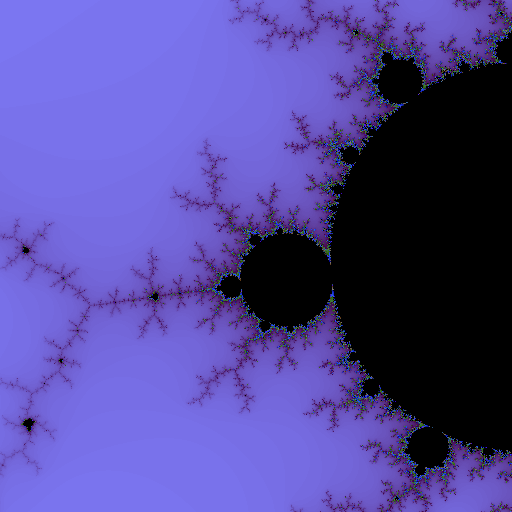
\includegraphics[scale=0.6]{mandel.png}
\end{center}
\label{fig:mandel}
\caption{Mandelbot Set picture generated on the GPU}
\end{figure}

The Mandelbrot Set is a mathematical construction over the
\emph{complex plane}, that is the two-dimensional plane of complex
numbers.  A particular point is said to be in the set if when the
following equation is repeatedly applied, $|z|$ does not diverge to
infinity:

\[
  z_{n+1} = c + z_n^2
\]

where $c$ is the point on the plane (a complex number), and $z_0 = c$.

In practice we iterate the equation for a fixed number of times, and
if it has not diverged at that point, then we declare the point to be
in the set.  Furthermore, to generate a pretty picture, we remember
the iteration at which each point diverged and map the iteration
values to some colour palette.

We know that $|z|$ will definitely diverge if it is greater than 2.
Now the magnitude of a complex number $x + iy$ is given by $\sqrt{x^2
  + y^2}$, so we can simplify the condition by squaring both sides,
giving us that divergence happens when $x^2 + y^2 > 4$.

Let's express this using \acc{}\footnote{the full sample code is in
  @mandel/mandel.hs@}.  First we want a type for complex numbers.
\acc{} lets us work with tuples, so we can represent complex numbers
as pairs of floating-point numbers.  As it happens, not all GPUs can
work with @Double@s, so we'll use @Float@:

\begin{haskell}
type F       = Float
type Complex = (F,F)
\end{haskell}

We'll be referring to @Float@ a lot, so the @F@ type synonym helps to
keep things readable.  Now, to calculate the next value of $z$ at a
given point $c$ looks like this:

\begin{haskell}
next :: Exp Complex -> Exp Complex -> Exp Complex
next c z = c `plus` (z `times` z)
\end{haskell}

\noindent We can't use the normal @+@ and @*@ operations here, because
there is no instance of @Num@ for @Exp Complex@---\acc{} doesn't know
how to add or multiply our complex numbers, so we have to define these
operations ourselves.  First, @plus@:

\begin{haskell}
plus :: Exp Complex -> Exp Complex -> Exp Complex
plus a b = ...
\end{haskell}

\noindent To sum two complex numbers we need to just sum the components.  But
how can we access the components?  We cannot pattern match on
@Exp Complex@.  There are a few different ways to do it, and we'll
explore them briefly.  \acc{} provides operations for selecting the
components of pairs in @Exp@, namely:

\begin{haskell}
fst :: (Elt a, Elt b) => Exp (a, b) -> Exp a
snd :: (Elt a, Elt b) => Exp (a, b) -> Exp b
\end{haskell}

\noindent So we could write plus like this:

\begin{haskell}
plus :: Exp Complex -> Exp Complex -> Exp Complex
plus a b = ...
  where
    ax = A.fst a
    ay = A.snd a
    bx = A.fst b
    by = A.snd b
\end{haskell}

\noindent but how do we construct the result?  We want to write
something like @(ax+bx, ay+by)@, but this has type @(Exp F, Exp F)@,
whereas we want @Exp (F,F)@.  Fortunately there is a function that can
perform exactly this conversion: @lift@ (see
\secref{accel-lift-unlift}).  So the result is:

\begin{haskell}
plus :: Exp Complex -> Exp Complex -> Exp Complex
plus a b = lift (ax+bx, ay+by)
  where
    ax = A.fst a
    ay = A.snd a
    bx = A.fst b
    by = A.snd b
\end{haskell}

In fact we could do a little better, since @A.fst@ and @A.snd@ are
just instances of @unlift@, and we could do them both in one go:

\begin{haskell}
plus :: Exp Complex -> Exp Complex -> Exp Complex
plus a b = lift (ax+bx, ay+by)
  where
    (ax, ay) = unlift a
    (bx, by) = unlift b
\end{haskell}

\noindent although unfortunately if you try this you will find that
there isn't enough type information for GHC, so we have to help it out
a bit:

\begin{haskell}
plus :: Exp Complex -> Exp Complex -> Exp Complex
plus a b = lift (ax+bx, ay+by)
  where
    (ax, ay) = unlift a :: (Exp F, Exp F)
    (bx, by) = unlift b :: (Exp F, Exp F)
\end{haskell}

\noindent We can go a little further, since \acc{} provides a useful
function that incorporates both the @lift@ and @unlift@.  For a
2-argument function, the right variant is called @lift2@:

\begin{haskell}
plus :: Exp Complex -> Exp Complex -> Exp Complex
plus = lift2 f
  where f :: (Exp F, Exp F) -> (Exp F, Exp F) -> (Exp F, Exp F)
        f (ax,ay) (bx,by) = (ax+bx,ay+by)
\end{haskell}

\noindent Unfortunately again we had to add the type signature to get
it to typecheck, but it does aid readability.  This is perhaps as
close to ``natural'' as we can get for this definition: the necessary
lifting and unlifting are confined to just one place.

We also need to define @times@, which follows the same pattern as
@plus@, although of course this time we are multiplying the two
complex numbers together:

\begin{haskell}
times :: Exp Complex -> Exp Complex -> Exp Complex
times = lift2 f
  where f :: (Exp F, Exp F) -> (Exp F, Exp F) -> (Exp F, Exp F)
        f (ax,ay) (bx,by)   =  (ax*bx-ay*by, ax*by+ay*bx)
\end{haskell}

So now we can compute $z_{n+1}$ given $z$ and $c$.  But we need to
think about the program as a whole: for each point, we need to iterate
this process until divergence, and then remember the number of
iterations at which divergence happened.  This creates a small
problem: GPUs are designed to do the \emph{same thing} to lots of
different data at the same time, whereas we want to do something
different depending on whether or not a particular point has diverged
or not.  So in practice we can't do what we would normally do in a
single-threaded language and iterate each point until divergence,
instead we have to find a way to apply the same operation to every
element of the array, for a fixed number of iterations.

In fact this is a common conundrum faced by the GPU programmer.  As a
rule of thumb, conditionals are ``bad'', because they cause \emph{SIMD
  divergence}.  This means that when the GPU hits a conditional
instruction, it first runs all the threads that take the true branch,
and then runs the threads that take the false branch.  Of course if
you have nested conditionals, the amount of parallelism rapidly
disappears.

We can't avoid \emph{some} kind of conditional in the mandelbrot
example, but we can make sure there is only a bounded amount of
divergence by having just one conditional per iteration, and a fixed
number of iterations.  The trick we use is to keep a pair @(z,i)@ for
every array element, where @i@ is the iteration at which that point
diverged.  At each iteration:

\begin{itemize}
\item Compute @z' = next c z@,
\item If it is greater than 4, then the result is @(z,i)@,
\item otherwise the result is @(z',i+1)@
\end{itemize}

\acc{} doesn't allow nested tuples, so we have to flatten the pair @z@
in @(z,i)@, to get @(x,y,i)@.  The operation we will apply to each
element therefore has this type:

\begin{haskell}
iter :: Exp Complex -> Exp (F,F,Int) -> Exp (F,F,Int)
iter c z = ...
\end{haskell}

\noindent The first thing to do is @unlift z@, so that we can access
the components of the triple, and then compute @z'@ by calling @next@:

\begin{haskell}
  let
     (x,y,i) = unlift z :: (Exp F, Exp F, Exp Int)
     z' = next c (lift (x,y))
  in
\end{haskell}

\noindent We had to use @lift@ to get @(x,y)@ back into the right form
for passing to @next@.  Now we have @z'@ we can do the conditional
test:

\begin{haskell}
  (dot z' >* 4.0) ?
     ( z
     , lift (A.fst z', A.snd z', i+1)
     )
\end{haskell}

\noindent where @dot@ computes $x^2 + y^2$; it follows the same
pattern as @plus@ and @times@ so we've omitted it here.  We are using
the infix @?@ operator for the conditional (\secref{accel-bool}).  In
the true case, we just return the original @z@,
whereas in the false case we return the new @z'@ and @i+1@.

The algorithm will need two arrays: one array of @c@ values which will
be constant throughout the computation, and a second array of @(z,i)@
values which will be recomputed by each iteration.  Our arrays are
2-dimensional arrays indexed by pixel coordinates, since the aim is to
generate a picture from the iteration values at each pixel.

The initial complex plane of @c@ values is generated by a function
@genPlane@:

\begin{haskell}
genPlane :: F -> F   -- X bounds of the view
         -> F -> F   -- Y bounds of the view
         -> Int      -- X resolution in pixels
         -> Int      -- Y resolution in pixels
         -> Acc ComplexPlane
\end{haskell}

\noindent its definition is rather long so we omit it here, but
essentially it is a call to @generate@
(\secref{accel-creating-arrays}).

From the initial complex plane we can generate the initial array of
@(z,i)@ values, which is done by initialising each @z@ to the
corresponding @c@ value, and @i@ to zero.  In the code this can be
found in the @mkinit@ function.

Now we can put the pieces together and write the code for the complete
algorithm:

\begin{haskell}
mandelbrot :: F -> F -> F -> F -- plane coordinates
           -> Int -> Int       -- view resolution
           -> Int              -- maximum iterations
           -> Acc (Array DIM2 (F,F,Int))

mandelbrot x y x' y' screenX screenY depth
  = iterate go (mkinit cs) !! depth
  where
    cs  = genPlane x y x' y' screenX screenY

    go :: Acc (Array DIM2 (F,F,Int))
       -> Acc (Array DIM2 (F,F,Int))
    go = A.zipWith iter cs
\end{haskell}

\noindent @cs@ is our static complex plane generated by @genPlane@.
The function @go@ performs one iteration, producing a new array of
@(z,i)@, and it is expressed by zipping @iter@ over both @cs@ and the
current array of @(z,i)@.  To perform all the iterations, we simply
call the ordinary list function @iterate@:

\begin{haskell}
iterate :: (a -> a) -> a -> [a]
\end{haskell}

\noindent and take the element at position @depth@, which corresponds
to the @go@ function having been applied @depth@ times.
